\chapter{Grundlagen} \label{ch:Grundlagen}

Dieses Kapitel dient zur Einführung der Schlüsselthemen der Masterthesis. Wesentliches Thema der Arbeit stellt das Optimierungsproblem (Multi-Mode) Resource-Constrained Project Scheduling Problem. Dieses (M)\ac{rcpsp} wird zunächst im Abschnitt \ref{sec:MRCPSP} erläutert. Metaheuristiken stellen eine generische Möglichkeit zur Lösung von Optimierungsproblemen dar. Abschnitt \ref{sec:Metaheuristiken} zeigt die Funktionsweise von verschiedenen Metaheuristiken auf. 

\section{(Multi-Mode) Resource-Constrained Project Scheduling Problem} \label{sec:MRCPSP}

Eines der am meisten verbreiteten Optimierungsprobleme stellt das Resource Constrained Project Scheduling Problem dar. Dieses Problem findet insbesondere bei der Projektplanung, aber auch in vielen Bereichen der Gegenwart einen realistischen Bezug. Das Problem bezieht sich auf das Finden von optimalen Schedules (dt. Zeitplänen) von festgelegten Projektablaufplänen, wobei die Aktivitäten erneuerbare Ressourcenanforderungen (z B. Maschinen oder menschliche Arbeitskraft) aufweisen. Optimale Schedules können nicht ohne Weiteres bestimmt werden, folglich müssen für einen gegebenen Projektplan alle Möglichkeiten durchiteriert werden. Dies stellt durch die Komplexität des Lösungsraums ein $\mathcal{NP}$-hartes Problem dar \cite[vgl.][S. 2]{kolisch_heuristic_1998}. Das \ac{rcpsp}-Basisproblem wird im Abschnitt \ref{subsec:MRCPSP_RCPSP} erläutert. \\

Das RCPSP sieht bei Aktivitäten nur eine Art der Ausführung vor. Zudem berück-sichtigt das Grundproblem keine nicht-erneuerbaren Ressourcen, wie z. B. Geldmengen oder Verbrauchsgüter, welche insbesondere in der Praxis und in Projekten wesentliche Bestandteile sind. Diese Aspekte werden in einer Problemerweiterung, nämlich dem Multi-Mode Resource-Constrained Project Scheduling Problem berücksichtigt \cite[vgl.][S. 596 f.]{wuliang_improved_2014}, welche im Abschnitt \ref{subsec:MRCPSP_MM} beleuchtet werden. \\

Um zunächst mögliche, wenn auch nicht optimale Lösungen zu erzeugen, wird unter anderem das Verfahren \ac{ssgs} eingesetzt. Dieses ermöglicht das Aufbauen von Schedules über das inkrementelle Erweitern von partiellen Schedules \cite[vgl.][S. 3]{kolisch_heuristic_1998}. \ac{ssgs} findet bei Heuristiken, aber auch in Metaheuristiken Verwendung \cite[vgl.][S. 3]{kolisch_heuristic_1998}. Beleuchtet wird das Konzept einschließlich der gängigen Heuristiken im Abschnitt \ref{subsec:SGS}. \\

In der Realität sind Unsicherheiten in Zeitplänen nicht abwegig. Diese können beispielsweise in Form von Verspätungen, aber auch über erhöhten Ressourcenverbrauch auftreten. Diese Thematik samt Möglichkeiten zum Umgang des Problems werden im Abschnitt \ref{subsec:MRCPSP_Unsicherheiten} erläutert. 


\subsection{Resource-Constrained Project Scheduling Problem} \label{subsec:MRCPSP_RCPSP}

% Einfach

Eines der am meisten behandelten Optimierungsprobleme stellt das \ac{rcpsp} dar. Das grundlegende \ac{rcpsp} behandelt das Finden von Schedules (dt. Zeitplänen) bei einem gegebenen Projektplan. Ein Projekt besteht aus einer Menge von Aktivitäten $J = \{ 0, ..., j, j + 1 \}$, wobei es sich $J_0$ und $J_{j+1}$ um Dummy-Aktivitäten handeln, welche den Projektstart bzw. das Projektende repräsentieren. Aktivitäten können untereinander in Beziehung stehen, sodass eine Aktivität $j \in J$ erst gestartet werden kann, wenn alle seine Vorgänger $P(j) \in 2^J$ fertiggestellt wurden. Diese besitzen im Grundproblem zudem eine feste Dauer $d_j \in \mathbb{N}_0$ und Ressourcenanforderungen $r_{j,k} \in \mathbb{N}_0$. Bei den Ressourcen wird zwischen erneuerbaren Ressourcenarten $K = \{1, ..., R\}$ unterschieden. Alle Ressourcenarten stehen innerhalb eines Projektes nur in limitierter Anzahl $R_{k} \in \mathbb{N}$ zur Verfügung, welche während der Projektausführung über die Aktivitäten aufgeteilt werden müssen. Für die Projektstart- und Ende-Aktivitäten gelten zudem $\forall \, k \in K: r_{j,k} = 0$ und $d_j = 0$. Diese Restriktion zeigt auf, dass keine Ressourcen- und Zeitanforderungen für die Aktivitäten gegeben sind. Zudem dürfen Aktivitäten nicht bei der Ausführung unterbrochen werden. \cite[vgl.][S. 1 ff.]{kolisch_heuristic_1998}. \\

Das Ziel des \ac{rcpsp} liegt darin, den Zeitplan mit der minimalsten Makespan (zu dt. Projektausführungsdauer) zu bestimmen. Formal wird die Zielfunktion des \ac{rcpsp} von \cite[S. 1]{kolisch_heuristic_1998} vergleichsweise wie folgt beschrieben:
\begin{align}
    \min \, F_{n+1} = \min \, C_{max} & \qquad \textit{es muss gelten:} \label{align:rcpsp_goal} \\
    \forall j \in J, h \in P_j:\, & F_h \leq F_j - d_j \label{align:rcpsp_constraint1} \\
    \forall k \in K, t \geq 0:\, & \sum_{j \in A(t)} r_{j,k} \leq R_k  \label{align:rcpsp_constraint2}
\end{align}
Die Menge der zum Zeitpunkt $t$ ausgeführten Aktivitäten wird über $A(t)$ angegeben. $F_j$ entspricht der Endzeit einer Aktivität $j \in J$. Eine Aktivität kann erst gestartet werden, wenn alle unmittelbaren Vorgänger abgeschlossen wurden (vgl. Formel \ref{align:rcpsp_constraint1}). Formel \ref{align:rcpsp_constraint2} gewährleistet, dass die Kapazitäten von den erneuerbaren Ressourcen zu jedem Zeitpunkt nicht überschritten werden dürfen. 

\begin{figure}[H]
    \centering
    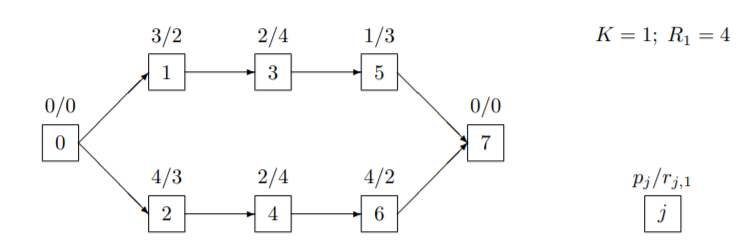
\includegraphics[width=1\textwidth]{assets/img/02_Grundlagen/ExampleProjectRCPSP_Plan.png}
    \caption{Graphen-Darstellung eines \ac{rcpsp} Beispiel-Projektplans mit $|J| = 8$ Aktivitäten} 
    \label{img:example_rcpsp}
    \source{\cite[][S. 2]{kolisch_heuristic_1998}}
\end{figure}

Abbildung \ref{img:example_rcpsp} stellt einen beispielhaften Projektplan mit $|J| = 8$ Aktivitäten als Knoten samt deren Ressourcen- und Zeitanforderungen dar. Diese stehen oberhalb der Knoten in der Schreibweise $d_j / r_{r,i}$. $J_0$ und $J_7$ entsprechen den Dummyknoten, welche keine Ressourcen- und Zeitanforderungen aufweisen. Die Kanten zeigen Beziehungen zu den Nachfolgeaktivitäten auf. Zudem steht eine erneuerbare Ressourcenart mit einer Kapazität von 4 Mengeneinheiten ($R_1 = 4$) zur Verfügung. 

\begin{figure}[H]
    \centering
    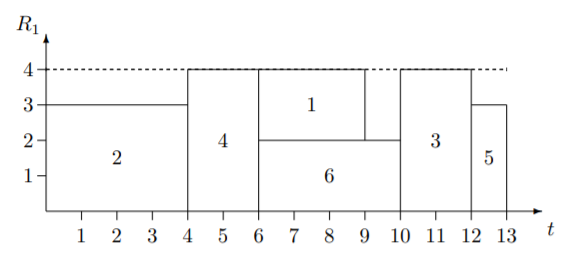
\includegraphics[width=0.8\textwidth]{assets/img/02_Grundlagen/ExampleProjectRCPSP_Schedule.png}
    \caption{Möglicher Zeitplan zum \ac{rcpsp} Beispiel-Projektplan} 
    \label{img:example_rcpsp_schedule}
    \source{\cite[][S. 2]{kolisch_heuristic_1998}}
\end{figure}
Ein möglicher Zeitplan zu dem Beispiel-Projektplan lässt sich in der Abbildung \ref{img:example_rcpsp_schedule} darstellen. Hierbei werden die Ressourcenanforderungen der Aktivitäten mit Berücksichtigung der Abhängigkeiten auf der Zeitachse gemäß deren Dauer zugeordnet. Die gestrichelte, horizontale Linie entspricht der maximalen Kapazität für die Ressource $K_1$, welche $R_1 = 4$ gleichkommt. Diese darf bei der Zeitplanung nicht überschritten werden. Der Makespan (dt. Zykluszeit) $C_{max} = 13$ des Zeitplans lässt sich über der Belegung der erneuerbaren Ressourcenarten über den Endzeitpunkt der letzten Aktivität $J_{j+1}$ ablesen. \\

Das \ac{rcpsp} wird als eine generalisierte Form des \ac{jsp} angesehen, welches als $\mathcal{NP}$-hartes Problem  klassifiziert wurde \cite[vgl.][S. 2]{kolisch_heuristic_1998}. Konkret bedeutet dies, dass das Finden des besten Zeitplans nur bei einem kleinen Lösungs-raum deterministisch über Bruteforcing möglich ist. Bei komplexeren Lösungsräumen sind jedoch zu viele Möglichkeiten vorhanden, als dass in absehbarer Zeit alle Kombinationen betrachtet werden können. \\
% Nicht-erneuerbare Ressourcen stellen zudem ein weiteres Problem dar, denn ungültige Lösungen können auftreten wenn zu einem Zeitpunkt keine nicht-erneuerbaren Ressourcen mehr zur Verfügung stehen. \\
\\
Für das zugrunde liegende Problem wurden (Meta-)Heuristiken und weitere intelligente Verfahren eingeführt, welche zur Findung von adäquaten Zeitplänen beim \ac{rcpsp} eingesetzt werden können \cite[vgl.][S. 2]{kolisch_heuristic_1998}. Der Fokus dieser Masterarbeit liegt bei den Metaheuristiken, welche im Abschnitt \ref{sec:Metaheuristiken} eingeführt werden.

\subsection{Multi-Mode Problemerweiterung} \label{subsec:MRCPSP_MM}

Das \ac{mrcpsp} basiert grundlegend auf dem \ac{rcpsp} und stellt somit eine Erweiterung des Basisproblems dar. \\

% Einfach

Im \ac{mrcpsp} steht für jede Aktivität $j \in J$ eine Menge von Modi $m \in M_j = \{ 1, ..., m_j \}$ zur Verfügung. Hierbei muss eine Aktivität in einem verfügbaren Modus $m \in M_j$ ausgeführt werden. Folglich liegen die Zeit- und Ressourcenanforderungen nicht  direkt bei den Aktivitäten, sondern bei den Modi. Die Zeitanforderung einer Aktivität $j \in J$ im Modus $m \in M_j$ wird über $d_{j,m}$ angegeben. Bei den verfügbaren Ressourcenarten kommen neben den erneuerbaren Ressourcenarten $K = \{1, ..., R\}$ auch nicht-erneuerbare Ressourcenarten $L = \{1, ..., C\}$ hinzu, welche über die Modi der Aktivitäten konsumiert werden. Die Menge an nicht-erneuerbaren Ressourcen stehen wie die erneuerbaren Ressourcen nur in limitierter Anzahl $C_l \in \mathbb{N}$ zur Verfügung. Die Ressourcenanforderungen einer Aktivität $j \in J$ im Modus $m \in M_j$ wird bei erneuerbaren Ressourcenarten über $r_{j,m,k}$ und bei nicht-erneuerbaren Ressourcenarten über $c_{j,m,l}$ angegeben. \cite[vgl.][S. 596 ff.]{wuliang_improved_2014} \\ 

Das Ziel des \ac{mrcpsp} ist identisch mit dem des \ac{rcpsp} und befasst sich ebenfalls mit dem Finden eines Zeitplans mit der minimalsten Projektausführungsdauer. Aufgrund der Problemerweiterung gegenüber dem \ac{rcpsp} sind zudem Anpassungen in der Zielfunktion erforderlich, welche \cite[vgl.][S. 597]{wuliang_improved_2014} aufführt: 
\begin{align}
    \min \, F_{n+1} = \min \, C_{max} & \qquad \textit{es muss gelten:} \label{align:mrcpsp_goal} \\
    \forall j \in J:\, & \sum_{m \in M_j} x_{j,m} = 1 \label{align:mrcpsp_constraint1}\\
    \forall j \in J, h \in P_j:\, & F_h \leq  F_j - \sum_{m \in M_j} x_{j,m} \cdot d_{j,m} \label{align:mrcpsp_constraint2} \\
    \forall k \in K, t \geq 0:\, & \sum_{j \in A(t)} \sum_{m \in M_j} x_{j,m} \cdot r_{j,k} \leq R_k  \label{align:mrcpsp_constraint3}
    \\
    \forall l \in C, t \geq 0:\, & \sum_{j \in J} \sum_{m \in M_j} x_{j,m} \cdot c_{j,l} \leq C_l  \label{align:mrcpsp_constraint4} 
\end{align}
$x_{j,m}$ stellt hierbei eine Entscheidungsvariable dar, die angibt, ob ein Modus $m \in M$ für die Aktivität $j \in M$ selektiert wurde. Sofern dies der Fall ist, entspricht $x_{j,m} = 1$, andernfalls $x_{j,m} = 0$. Die Beschränkung in \ref{align:mrcpsp_constraint1} nutzt diese Entscheidungsvariable, um sicherzustellen, dass für jede Aktivität immer ein Modus ausgewählt wurde. Die Beschränkung aus  \ref{align:mrcpsp_constraint2} stellt die Erweiterung aus \ref{align:rcpsp_constraint1} dar und soll weiterhin sicherstellen, dass die Abhängigkeitsbeziehungen zwischen den Aktivitäten für alle ausgewählten Modis eingehalten werden. \ref{align:mrcpsp_constraint3} berücksichtigt ebenfalls nun die Modusauswahl und stellt sicher, dass die Kapazität an erneuerbaren Ressourcen zu keinem Zeitpunkt überschritten werden darf. Die Beschränkung aus \ref{align:mrcpsp_constraint4} stellt sicher, dass zu keinem Zeitpunkt mehr nicht-erneuerbare Ressourcen konsumiert werden, als zur Verfügung stehen. \\

\begin{figure}[H]
    \centering
    \noindent\makebox[\textwidth]{%
    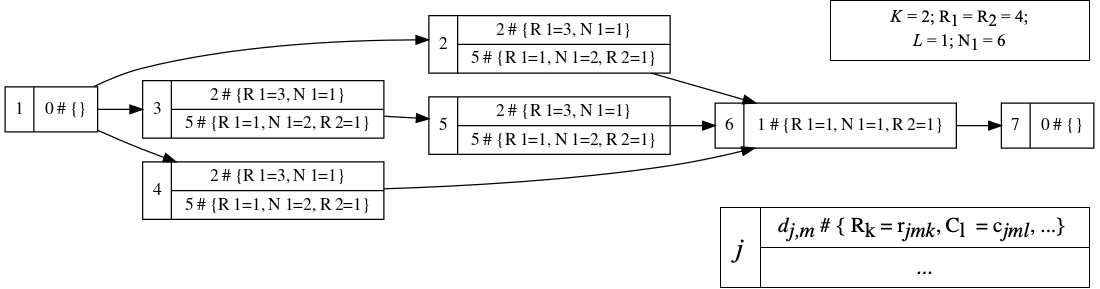
\includegraphics[width=1.1\textwidth]{assets/img/02_Grundlagen/ExampleProjectMRCPSP_Plan.png}
    }
    \caption{Graphen-Darstellung eines \ac{mrcpsp} Beispiel-Projektplans mit $|J| = 7$ Aktivitäten} 
    \label{img:example_mrcpsp}
    \source{Eigene Darstellung}
\end{figure}

Abbildung \ref{img:example_mrcpsp} zeigt eine grafische Darstellung eines \ac{mrcpsp} Beispielprojektes mit 7 Aktivitäten dar, wobei $J_0$ und $J_7$ die Dummy-Knoten entsprechen. Innerhalb der Aktivitätsknoten befinden sich zudem die zugehörigen ausführbaren Modi mit deren Zeit- und Ressourcenanforderungen. Die Aktivitäten $J_2 \, ... \, J_4$ können jeweils in zwei verschiedenen Versionen ausgeführt werden, sofern die Beschränkungen eingehalten werden. \\

\begin{figure}[H]
    \centering
    \noindent\makebox[\textwidth]{%
    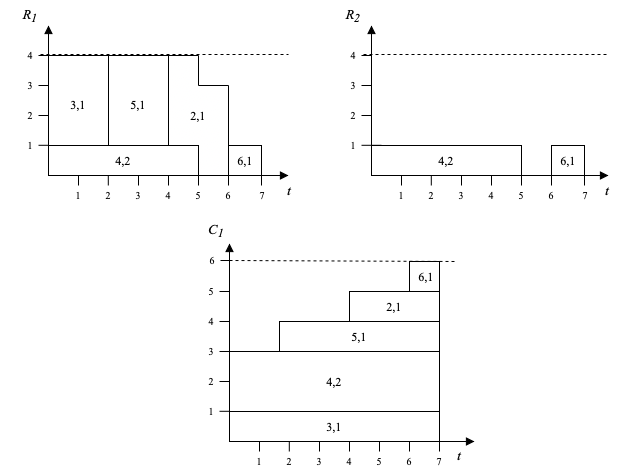
\includegraphics[width=1.1\textwidth]{assets/img/02_Grundlagen/ExampleProjectMRCPSP_Schedule.png}
    }
    \caption{Möglicher Zeitplan zum \ac{mrcpsp} Beispiel-Projektplan} 
    \label{img:example_mrcpsp_schedule}
    \source{Eigene Darstellung}
\end{figure}

Abbildung \ref{img:example_mrcpsp_schedule} zeigt für den \ac{mrcpsp} Beispiel-Projektplan eine optimale Belegung aller Ressourcenarten auf. In der Grafik wurden für alle Aktivitäten auch die zugehörigen Modi gekennzeichnet. Der Makespan für diesen (optimalen) Zeitplan liegt bei $C_{max} = 7$. Dadurch, dass sich nicht-erneuerbare Ressourcen $C_l$ nicht regenerieren, wird dieses Verhalten bei der Ressourcenbelegungsabbildung dahingehend berücksichtigt, dass jede gestartete Aktivität bis zum Projektende andauert. Es lässt sich erkennen, dass für das Beispiel am Projektende keine nicht-erneuerbaren Ressourcen mehr zur Verfügung stehen und folglich das Ausführen von weiteren Aktivitäten über den zweiten Modus zu invaliden Schedules führen würde. Der Verbrauch von nicht-erneuerbaren Ressourcen wäre im zweiten Modus bei allen Aktivitäten im Beispiel-Projektplan höher als bei dem ersten Modus und folglich würde die Grenze $C_l$ überschritten werden. \\
Aufgrund der nicht-erneuerbaren Ressourcenanforderungen und der Möglichkeit, Aktivitäten über verschiedene Modis auszuführen bewies \cite[S. 3 f.]{kolisch_local_1997}, dass sich das \ac{mrcpsp} nicht um ein $\mathcal{NP}$-hartes, sondern sogar um ein $\mathcal{NP}$-vollständiges Problem handelt. Dies ist dann der Fall, wenn mehr als zwei nicht-erneuerbare Ressourcenarten $|L| \geq 2$ und nicht-Dummy Aktivitäten in mehr als zwei Modi $\exists j \in J \, / \, \{ J_0, J_{j+1} \}: |M_j| \geq 2$ ausgeführt werden können \cite[vgl.][S. 3 f.]{kolisch_local_1997}. Durch die Auswahl der Modi wird direkt der Verbrauch an nicht-erneuerbaren Ressourcen beeinflusst. Die nicht-erneuerbaren Ressourcenanforderungen können nach Selektion der Modi die verfügbare Kapazität $C_l$ überschreiten, was ein Schedule gemäß Bedingung \ref{align:mrcpsp_constraint4} ungültig macht. \\

Heuristiken basierend auf prioritätsbasierten Regeln stellen für die Berechnung von Schedules auch beim \ac{mrcpsp} eine wichtige Technik für das Finden von adäquaten, wenn aber nicht optimalen Lösungen dar. Diese werden im Abschnitt \ref{subsec:SGS} genauer beleuchtet. Bei komplexen Projekten mit mehr als 20 Aktivitäten kommen Heuristiken an ihre Grenzen. Folglich werden Metaheuristiken eingesetzt, welche mittels lokaler Suche versuchen die optimale Lösung zu finden. Viele Metaheuristiken benötigen initiale Lösungen, wofür Heuristiken jedoch eine gute Basis darstellen. \cite[vgl.][S. 69 f.]{lova_multi-mode_2006} 
\subsection{Serial Schedule Generation Scheme} \label{subsec:SGS}

\acp{sgs} stellen für das (M)\ac{rcpsp} wesentliche Techniken zur Erzeugung von Zeitplänen dar. Die am häufigsten in der Literatur verwendeten \acp{sgs} sind \acfp{ssgs} und \acfp{psgs}. Das Prinzip eines \ac{sgs} liegt darin,  vollständige Zeitpläne inkrementell über partielle Zeitpläne aufzubauen. Ein partieller Schedule entspricht einem Zeitplan, welcher unvollständig ist und nicht alle Aktivitäten berücksichtigt, sondern nur eine Teilmenge von Aktivitäten. \cite[vgl.][S. 3 f.]{kolisch_heuristic_1998}\\

Die beiden \ac{sgs} Varianten unterscheiden sich bei der Inkrementierungsweise voneinander. Beim \ac{ssgs} werden $n$ Phasen durchlaufen, wobei in jeder Phase eine Aktivität selektiert wird. Bei dem \ac{psgs} werden bis zu $n$ Phasen durchlaufen. Zu jedem Aktivitätsendzeitpunkt wird überprüft, welche Aktivitäten ausgewählt werden können. Während das \ac{ssgs} aktivitätsinkremental funktioniert, agiert das \ac{psgs} zeitinkremental. \cite[vgl.][S. 3 f.]{kolisch_heuristic_1998}\\

Im Rahmen der Masterthesis wird vermehrt das \ac{mrcpsp} behandelt, welches in Kombination mit dem \acf{psgs} nicht immer eine optimale Lösung darstellt \cite[vgl.][S. 911 f.]{alcaraz_solving_2003} \cite[vgl.][S. 5 f.]{kolisch_heuristic_1998} . Folglich beschränkt sich diese Arbeit auf das \ac{ssgs}. 

\begin{lstlisting}[caption={\ac{ssgs}-Algorithmus (Quelle: \cite[S. 3]{kolisch_heuristic_1998}}), label=lst:sgsalgorithm, mathescape=true, inputencoding={utf8}, extendedchars=false, escapeinside=``]
Init: $F_0$, $S_0 = $ {0},
for g = 1 to n do
    Berechne $\mathcal{D}_g, \mathcal{F}_g, \tilde{\mathcal{R}}_k(t) \, (k \in \mathcal{K}; t \in \mathcal{F}_g)$ 
    W`ä`hle ein $j \in \mathcal{D}$ aus
    $EFT_j$ = $\max_{h \in \mathcal{P}_j} \{ F_h \} + p_j$
    $F_j$ = $\min \{ t \in [EFT_j - p_j, LFT_j - p_j] \cap \mathcal{F}_g | r_{j,k} \leq R_k(\tau), k \in \mathcal{K}, \tau \in [t, t + p_j [\cap \mathcal{F}_g\} + p_j $
    $\mathcal{S}_g$ = $\mathcal{S}_{g - 1} \cup \{ j \}$
$F_{n+1}$ = $\max_{h \in \mathcal{P}_{n+1}} \{ F_h \}$  
\end{lstlisting}

Listing \ref{lst:sgsalgorithm} stellt den \ac{ssgs}-Algorithmus aus dem Manuskript von \cite{kolisch_heuristic_1998} dar. Hierbei wird in jeder Phase $g$ die Mengen $\mathcal{S}_g$ und $\mathcal{D}_g$ berechnet. Die Menge $\mathcal{S}_g$ beinhaltet bereits berücksichtigte Aktivitäten, während $\mathcal{D}_g$ die selektierbaren Aktivitäten für die Phase $g$ beinhaltet. Die Menge $\mathcal{F}_g$ beinhaltet zu $\mathcal{S}_g$ die Endzeiten der einzelnen Aktivitäten. $\tilde{\mathcal{R}}_k(t)$ gibt die Anzahl noch verfügbarer erneuerbarer Ressourcen für die Ressourcenart $k$ zum Zeitpunkt $t$ an. \cite[vgl.][S. 3 f.]{kolisch_heuristic_1998}\\

Abbildung \ref{img:example_ssgs_application} zeigt auf, wie \ac{ssgs} auf einen Projektplan angewendet werden kann, um eine mögliche Lösung für das \ac{rcpsp} zu erhalten. Die Auswahl der Aktivität $j$ aus $\mathcal{D}_g$ erfolgte in dem Beispiel willkürlich. 

\begin{figure}[H]
    \centering
    \noindent\makebox[\textwidth]{%
    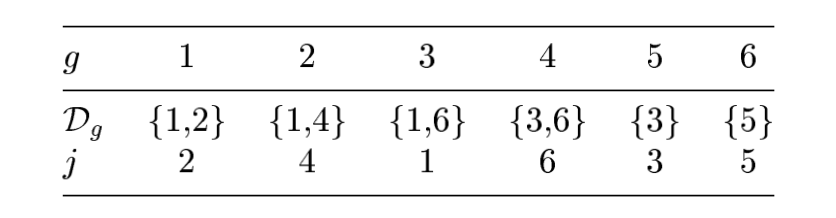
\includegraphics[width=0.6\textwidth]{assets/img/02_Grundlagen/ExampleSSGS.png}
    }
    \caption{\acs{ssgs}-Anwendung auf den RCPSP Beispiel-Projektplan von Abbildung \ref{img:example_rcpsp} zur Erstellung des Zeitplans aus Abbildung \ref{img:example_rcpsp_schedule}}
    \label{img:example_ssgs_application}
    \source{\cite[vgl.][S. 3]{kolisch_heuristic_1998}}
\end{figure}

Aus dem Listing \ref{lst:sgsalgorithm} heraus lassen sich weitere Kennziffern von Aktivitäten innerhalb eines Projektplans erkennen. Im Algorithmus wurden \ac{EFT} und \ac{LFT} verwendet. Diese und \ac{EST} und \ac{LST} sind wesentlich für viele prioritätsbasierte Aktivitätsregeln (vgl. Abschnitt \ref{subsec:SGS_Aktivitaeten}) und für die Robustheitsberechnungen (vgl. Abschnitt \ref{subsec:Praediktive_Methoden}) und werden in der Tabelle \ref{tab:cmr_kennziffern} eingeführt. \\

\begin{table}[H]
\centering
\begin{adjustbox}{width=0.9\columnwidth,center}
\begin{tabular}{|l|l|l|}
\hline
Abk. & Beschreibung \cite[vgl.][S. 126]{burke_project_1999} & Formel \cite[vgl.][S. 127 ff.]{burke_project_1999} \\ \hline
EST  & \begin{tabular}[c]{@{}l@{}}Earliest Starting Time\\ (dt. frühster Startzeitpunkt)\\ stellt den frühstmöglichen Start-\\ zeitpunkt einer Aktivität $j$ dar. \end{tabular}  & $EST_j = \max_{h \in P(j)} \{ EFT(h) \}$ \\ \hline
EFT  & \begin{tabular}[c]{@{}l@{}}Earliest Finishing Time\\ (dt. frühster Endzeitpunkt) \\ stellt den frühstmöglichen End-\\ zeitpunkt einer Aktivität $j$ dar. \end{tabular} & $EFT_j = EST_j + d_j $\\ \hline
LST  & \begin{tabular}[c]{@{}l@{}}Latest Starting Time\\ (dt. spätester Startzeitpunkt)\\ stellt den spätesten Startzeit-\\ punkt einer Aktivität $j$ dar, ohne \\ dass das Projekt in Verzug kommt. \end{tabular} & $LST_j = LFT_j - d_j$ \\ \hline
LFT  & \begin{tabular}[c]{@{}l@{}}Latest Finishing Time\\ (dt. spätester Endzeitpunkt)\\ stellt den spätesten Endzeit-\\ punkt einer Aktivität $j$ dar,\\ ohne dass das Projekt in \\ Verzug kommt. \end{tabular}  & $LFT_j = \min_{h \in P(j)} \{ LST(h) \}$ \\ \hline
\end{tabular}
\end{adjustbox}
\caption{Kennziffern der kritischen Pfadmethode}
\source{In Anlehnung an \cite{burke_project_1999}}
\label{tab:cmr_kennziffern}
\end{table}

\subsubsection{Aktivitäts- und Moduslisten} \label{subsec:SGS_Darstellung}  
Aktivitäts- und Moduslisten sind wesentliche Techniken zur Repräsentation von Lösungen für das (M)\ac{rcpsp}. Insbesondere Metaheuristiken nutzen diese Art der Repräsentation, um aus den Listen Zeitpläne zu transferieren \cite[vgl.][S. 10]{rezaeian_using_2015}, \cite[vgl.][S. 602]{wuliang_improved_2014}, \cite[vgl.][S. 2370]{li_solving_2013}. \\

Zeitpläne im \ac{rcpsp} lassen sich über Aktivitätslisten  $\lambda = \langle j_1, j_2, ..., j_n \rangle$ darstellen. Die Reihenfolge der Aktivitäten entspricht die der Planungsreihenfolge. Folglich müssen die Abhängigkeiten der Aktivitäten zueinander innerhalb der Aktivitätsliste $\lambda$ eingehalten werden. Im Beispiel der Abbildung \ref{img:example_rcpsp_schedule} entspricht die Aktivitätsliste $\lambda = \langle 2, 4, 1, 6, 3, 5 \rangle$. \cite[vgl.][S. 3 f.]{kolisch_heuristic_1998} \\

Für das \ac{mrcpsp} müssen zudem Modi der zugehörigen Aktivitäten berücksichtigt werden. Hierfür werden zusätzlich zu den Aktivitätslisten auch Moduslisten eingesetzt. Eine Modusliste $\mu = \langle m_1, m_2, ..., m_n \rangle$ berücksichtigt ebenfalls die Planungsreihenfolge. Die Länge der Modusliste entspricht der Länge der Aktivitätsliste $|\mu| \equiv |\lambda|$. Folglich können über Aktivitäts- und Moduslisten die Aktivitäten und Modi über die Positionierung zugeordnet werden \cite[vgl.][S. 908]{sebt_efficient_2015}. Für das Beispiel aus Abbildung \ref{img:example_mrcpsp_schedule} entspricht die Aktivitäts- und Modusliste das Tupel $(\lambda, \mu) = (\langle 1, 3, 4, 5, 2, 6, 7 \rangle, \langle 1, 1, 2, 1, 1, 1, 1 \rangle)$. Abbildung \ref{img:ActivityModeListExample} illustriert dieses Beispiel. \\

\begin{figure}[H]
    \centering
    \noindent\makebox[\textwidth]{%
    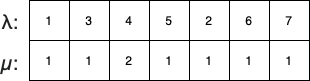
\includegraphics[width=0.45\textwidth]{assets/img/02_Grundlagen/ActivityModeListExample.png}
    }
    \caption{Darstellung der Aktivitäts- und Modusliste $(\lambda, \mu)$ für das MRCPSP Beispiel-Projektplan} 
    \label{img:ActivityModeListExample}
    \source{Eigene Darstellung}
\end{figure}

Eine Lösung für das \ac{mrcpsp} entspricht dem Tupel $I = (\lambda, \mu)$. Für jeden Projektplan existiert mindestens eine optimale Lösung mit der kürzesten Projektdauer $I^* = (\lambda^*, \mu^*)$ \cite[vgl.][S. 4]{kolisch_heuristic_1998}. Das Ziel der (Meta-)Heuristiken liegt darin, die optimale Lösung $I^*$ zu finden oder dieser zumindest sehr nahezukommen. Hierfür müssen Aktivitäts- und Moduslisten ausgewählt, evaluiert und anschließend weitergesucht werden. Abschnitt \ref{subsec:SGS_Aktivitaeten} befasst sich mit Heuristiken zum Finden von Aktivitätslisten, Abschnitt \ref{subsec:SGS_Modi} mit dem Finden von Moduslisten. 

\subsubsection{Prioritätsbasierte Regeln für Aktivitäten} \label{subsec:SGS_Aktivitaeten}

Das \acl{ssgs} stellt eine bedeutende Technik zur Erzeugung von Aktivitätslisten dar. Hierbei wird in jeder Phase $g$ eine Aktivität $j$ aus den möglichen Aktivitäten $\mathcal{D}_g$ ausgewählt. Die Auswahl der Aktivität $j \in \mathcal{D}_g$ gilt es mittels prioritätsbasierten Regeln zu bestimmen. \cite[vgl.][S. 5]{kolisch_heuristic_1998}\\

Prioritätsbasierte Regeln bestehen aus zwei Komponenten, nämlich einer Prioritätswertfunktion $v(j)$ und einem Auswahlparameter $extr$. Die Prioritätswertfunk-tion für Aktivitäten ist über $v: \mathcal{D}_g \rightarrow \mathbb{R}_0$ gemappt und wird über die Prioritätsregeln definiert. Die Funktion gibt für eine mögliche Aktivität $j \in \mathcal{D}_g$ den entsprechenden Prioritätswert gemäß der Regel an. Der Auswahlparameter $extr \in \{ \text{MIN}, \text{MAX} \}$ bestimmt das Extremum. In jeder Phase wird eine Aktivität ausgewählt, die mit dem zugehörigen Prioritätswert dem Extremum aller möglichen Aktivitäten entspricht. Sofern mehrere Aktivitäten dem Extremwert entsprechen, muss eine weitere Heuristik eingeführt werden, wie die Auswahl über die geringste Aktivitätsnummer. \cite[vgl.][S. 6 f.]{schirmer_parameterized_1997}

% Beispiel Auswahl über Prioritätswert

\begin{table}[H]
\centering
\begin{tabular}{r|lll}
Abkürzung & Name & \multicolumn{1}{c}{\begin{tabular}[c]{@{}c@{}}Prioritätsregel-\\funktion $v(j)$\end{tabular}} & \multicolumn{1}{c}{\begin{tabular}[c]{@{}c@{}}Auswahl-\\parameter $extr$\end{tabular}} \\ \hline
GRPW & Greatest Rank Positional Weight & $d_j + \sum_{i \in S(j)} d_i $ & MAX \\
LFT & Latest Finish Time & $LFT_j $ & MIN \\
LST & Latest Start Time & $LST_j $ & MIN \\
MSLK & Minimum Slack & $LFT_j - EFT_j$ & MIN \\
MTS & Most Total Successors & $|S(j)| $ & MAX \\
\end{tabular}
\caption{Prioritätsregeln für Aktivitäten}
\label{tab:ActivityRules}
\source{\cite[vgl.][S. 6]{kolisch_heuristic_1998}}
\end{table}

Die in Tabelle \ref{tab:ActivityRules} aufgeführten etabilierten Regeln werden genutzt, um anhand der Prioritätsregelfunktion $v(j)$ gemäß Auswahlparameter $extr$ die zugehörige Aktivität $j$ auszuwählen. Tabelle \ref{tab:ActivityRulesExample} zeigt ein Beispiel bei Anwendung einer beliebigen Prioritätsregelfunktion $v(j)$ auf. Sofern der Auswahlparameter $extr = \text{MAX}$ entspricht, wird in der Phase $g$ die Aktivität 3 ausgewählt, bei $extr = \text{MIN}$ die Aktivität 2.  
 
\begin{table}[H]
\centering
\begin{tabular}{r|c|c|c|c}
$j \in \mathcal{D}_g$ & 1 & 2 & 3  & 4 \\ \hline
$v(j)$ & 5 & 3 & 12 & 4
\end{tabular}
\caption{Beispiele von Prioritätswerten von den möglichen Aktivitäten $j \in \mathcal{D}_g$ einer Phase $g$}
\label{tab:ActivityRulesExample}
\source{Eigene Darstellung}
\end{table}


\subsubsection{Selektionsregeln für Modi} \label{subsec:SGS_Modi}
Um beim \ac{mrcpsp} Zeitpläne zu erzeugen, müssen neben den Aktivitätslisten auch Moduslisten generiert werden. Des Weiteren besteht beim \ac{mrcpsp} die Problematik, dass bei Anwendung der Prioritätsregeln für eine Aktivität mehrere Modi mit unterschiedlichen Ressourcen- und Zeitanforderungen zur Verfügung stehen. Folglich werden Selektionsregeln für Modi benötigt, welche analog zu den Prioritätsregeln für Aktivitäten funktionieren. \\


\begin{table}[H]
\centering
\resizebox{\textwidth}{!}{%
\begin{tabular}{r|lll}
Abkürzung & Name & \multicolumn{1}{c}{\begin{tabular}[c]{@{}c@{}}Selektionsregel-\\funktion $s(j, m)$\end{tabular}} & \multicolumn{1}{c}{\begin{tabular}[c]{@{}c@{}}Auswahl-\\parameter $extr$\end{tabular}} \\ \hline
LPSRD & Least Product Sum of Res. and Dur. & $\sum_{l=1}^{|L|} (c_{j,m,l} \cdot d_{j,m})$ & MIN \\
LRP & Least Resource Proportion & $\max (\frac{r_{j,m,k}}{|K|})$ & MIN \\
LRS & Least Sum of Non-renewable Resource & $\sum_{l=1}^{|L|}  \frac{c_{j,m,l}}{R^v_k}$ & MIN \\
LTRU & Least Total Resource Usage & $\sum_{l=1}^{|L|} c_{j,m,l}$ & MIN \\
SFM & Shortest Feasible Mode & $d_{j,m}$ & MIN \\

\end{tabular}
}%
\caption{Selektionsregeln für Modi}
\label{tab:ModeRules}
\source{\cite[vgl.][S. 5046]{chen_entropy-based_2014}}
\end{table}

Die in Tabelle \ref{tab:ModeRules} aufgeführten etabilierten Regeln werden genutzt, um anhand der Selektionsregelfunktion $s(j, m)$ gemäß Auswahlparameter $extr$ den zugehörigen Modus $m \in M_j$ einer Aktivität $j$ auszuwählen. Tabelle $\ref{tab:ModesRulesExample}$ zeigt ein Beispiel bei Anwendung einer beliebigen Prioritätsregelfunktion $v(j)$ und Selektionsregelfunktion $s(j, m)$ auf. Um die Aktivitätsregelfunktion anwenden zu können, müssen vorher die Modi selektiert werden \cite[vgl.][S. 5046]{chen_entropy-based_2014}. Die Selektion der Modi und Aktivitäten geschieht im Beispiel über $extr = \text{MAX}$. Für alle möglichen Aktivitäten der Phase $j \in \mathcal{D}_g$ wird somit der erste Modus ausgewählt. Im Anschluss können die Aktivitäten über die Prioritätsregeln ausgewählt werden (vgl. Abschnitt \ref{subsec:SGS_Aktivitaeten}). 


\begin{table}[H]
\centering

\begin{tabular}{r|cc|cc|cc|cc}
$j \in \mathcal{D}_g$  & \multicolumn{2}{c|}{1} & \multicolumn{2}{c|}{2} & \multicolumn{2}{c|}{3} & \multicolumn{2}{c}{4} \\ \hline
$m \in M_j$ & \multicolumn{1}{c|}{1} & 2 & \multicolumn{1}{c|}{1} & 2 & \multicolumn{1}{c|}{1} & 2 & \multicolumn{1}{c|}{1} & 2 \\ \hline
$s(j, m)$                 & \multicolumn{1}{c|}{5} & 3 & \multicolumn{1}{c|}{2} & 1 & \multicolumn{1}{c|}{5} & 4 & \multicolumn{1}{c|}{7} & 7 \\ \hline
$v(j)$                      & \multicolumn{2}{c|}{5} & \multicolumn{2}{c|}{3} & \multicolumn{2}{c|}{12} & \multicolumn{2}{c}{2} 
\end{tabular}%

\caption{Beispiele von Prioritäts- und Selektionswerten von den möglichen Aktivitäten $j \in \mathcal{D}_g$ und Modis der Aktivitäten einer Phase $g$}
\label{tab:ModesRulesExample}
\source{Eigene Darstellung}
\end{table}

\subsubsection{Sampling als Multi Pass Methode} \label{subsec:SGS_RBBRS}

Das Anwenden der Aktivitäts- und Modusregeln führt innerhalb eines \ac{ssgs} zu einem einzigen Zeitplan und wird somit als eine Single Pass Methode klassifiziert \cite[vgl.][S. 6]{kolisch_heuristic_1998}. Das Anwenden dieser Heuristiken führt bei gleichbleibendem Input zudem immer zu identischen Ergebnissen und sind folglich deterministisch \cite[vgl.][S. 4]{schirmer_parameterized_1997}. Dennoch besteht das Interesse eine breitere Menge an möglichen Zeitplänen zu untersuchen, um durchaus bessere Ergebnisse als das direkte Anwenden der Regeln zu erhalten.\\

Unter Multi Pass Methoden werden wiederum Verfahren bezeichnet, die in der Lage sind, mehrere Zeitpläne zu generieren. Hierunter fallen Verfahren, wie das Anwenden von mehreren Regeln, aber auch das Sampling. Für jede mögliche Aktivität einer Phase $j \in \mathcal{D}_g$ und deren jeweiligen Modi $m \in M_j$ ist hierbei ein Wahrscheinlichkeitswert gemäß Funktion $p(x) \in [0, 1]$ vorgesehen, welche für die Entscheidungsmenge aufkommuliert stets 1 ergeben muss. Aus der Entscheidungsmenge wird im Anschluss gemäß der Wahrscheinlichkeit die Aktivität bzw. der Modus ausgewählt. Die Wahrscheinlichkeitsfunktion $p(x)$ wird anhand von Sampling Methoden definiert. \cite[vgl.][S. 7 f.]{kolisch_heuristic_1998} Aufgrund der Einfachheit beziehen sich die Formeln der folgenden vorgestellten Sampling Methoden nur auf die Aktivitätsauswahl. Diese lassen sich jedoch ohne weiteres auch auf die Modusauswahl ableiten. \\

Die einfachste Sampling Methode ist \ac{RS}. Hierbei ist die Wahrscheinlichkeit $p(x)$ innerhalb der Entscheidungsmenge gleichverteilt $p(j) = \dfrac{1}{|\mathcal{D}_g|}$. \cite[vgl.][S. 7]{kolisch_heuristic_1998} Hierbei werden Prioritäts- und Selektionregeln ignoriert und gänzlich zufällige Zeitpläne erzielt. \\

Eine weitere Sampling Methode ist \ac{BRS}. Die Wahrscheinlichkeit $p(x)$ hängt hierbei direkt von der Prioritäts- und Selektionsregel ab $p(j) = \dfrac{v(j)}{\sum_{i \in \mathcal{D}_g} v(i)}$. \cite[vgl.][S. 7]{kolisch_heuristic_1998} \\

Über \ac{RBRS} ist es zudem möglich, die Wahrscheinlichkeit $p(x)$ über einen Regretwert (dt. Reuewert) zu beeinflussen \cite[vgl.][S. 12]{schirmer_parameterized_1997}. Dies führt dazu, dass die Aktivitäts- und Moduslisten gemäß der Prioritäts- und Selektionsregeln mehr oder weniger variieren können. Die Wahrscheinlichkeit $p(x)$ lässt sich über die folgenden Funktionen gemäß \cite[vgl.][S. 12]{schirmer_parameterized_1997} definieren: 
\begin{align}
    v'(j) &= 
    \left\{\begin{array}{ll} 
        \max_{i \in \mathcal{D}_n}(v(i)) - v(j) & \text{wenn extr = min} \\
        v(j) - \min_{i \in \mathcal{D}_n}(v(i)) & \text{wenn extr = max} \\
     \end{array}\right.  \\
    v''(j) &= (v'(j) + \epsilon)^\alpha  \\
    p(j) &= \frac{v''(j)}{\sum_{i \in D_n} v''(i)}
\end{align}

$v'(j)$ und $v''(j)$ stellen die Regrets dar. Beim \ac{RBRS} werden die Regrets zudem mit $\epsilon = \mathbb{R}_{>0}$ und $\alpha = \mathbb{R}_{\geq0}$ parametrisiert. $\epsilon$ garantiert, dass $v''(j) \neq 0$. Dies ist relevant, um innerhalb der Wahrscheinlichkeitsfunktion $p(x)$ Divisionen durch 0 zu vermeiden. $\alpha$ regelt den Einfluss der Prioritäts- und Selektionsregelfunktion auf den Wahrscheinlichkeitswert. Bei einem hohen Wert verstärkt sich der Einfluss, bei einem niedrigen Wert verringert sich dieser. Bei $\alpha = 0$ ist die Prioritäts- und Selektionsregelfunktion irrelevant und folglich sind die Wahrscheinlichkeiten innerhalb der Entscheidungsmenge gleichverteilt, identisch zum \ac{RS}. Bei $\alpha = \infty$ sind die Wahrscheinlichkeiten so angeordnet, dass die Aktivität oder der Modus deterministisch ausgewählt werden kann, identisch zur Single Pass Methode. \cite[vgl.][S. 12 f.]{schirmer_parameterized_1997} \\

Die Funktionsweise der vorgestellten Multi Pass Samplingverfahren lassen sich in Tabelle \ref{tab:ExampleSampling} aufbauend auf dem Beispiel aus Abschnitt \ref{subsec:SGS_Aktivitaeten} verdeutlichen. Für dieses Beispiel liegt der Extremwert für die zu betrachtende Prioritätsregel bei $extr = \text{MAX}$. Sofern \ac{RBRS} als Sampling-Methode ausgewählt wurde, so wird z. B. die Aktivität 3 mit einer 80 prozentigen Wahrscheinlichkeit selektiert. Wenn $\alpha = \infty$, dann wird das Ergebnis gemäß der regelbasierten Single Pass Methode deterministisch ausgewählt.  




\begin{table}[H]
\centering
\begin{tabular}{r|l|l|l|l}
$j \in \mathcal{D}_g$                      & \multicolumn{1}{c|}{1} & \multicolumn{1}{c|}{2} & \multicolumn{1}{c|}{3}  & \multicolumn{1}{c}{4} \\ \hline
$v(j)$                                     & \multicolumn{1}{c|}{5} & \multicolumn{1}{c|}{3} & \multicolumn{1}{c|}{12} & \multicolumn{1}{c}{4} \\ \Xhline{2\arrayrulewidth}
\acf{RS} & 0.25                   & 0.25                   & 0.25                    & 0.25                  \\ \hline
\acf{BRS}& 0,21                   & 0,13                   & 0,50                    & 0,16                  \\ \hline
\acf{RBRS} & 0,10                   & 0,03                   & 0,80                    & 0,07                  \\ \hline
\ac{RBRS} mit $\alpha = 0$                      & 0.25                   & 0.25                   & 0.25                    & 0.25                  \\ \hline
\ac{RBRS} mit $\alpha = \infty$                      & 0.00                   & 0.00                   & 1.00                    & 0.00                 
\end{tabular}
\caption{Selektionswahrscheinlichkeiten $p(j)$ für die vorgestellten Sampling-Verfahren mit $|\mathcal{D}_g| = 4$ und $extr = \text{MAX}$ }
\label{tab:ExampleSampling}
\source{In Anlehnung an \cite[vgl.][S. 8]{kolisch_heuristic_1998}}
\end{table}

\subsection{Unsicherheiten} \label{subsec:MRCPSP_Unsicherheiten}

Insbesondere in der Realität ist es möglich, dass Unsicherheiten auftreten können. Dies kann der Fall sein, wenn Events, wie der Ausfall von Maschinen, die Erkrankung von Mitarbeitern, die Fehleinschätzung bei der Planung usw. auftreten \cite[vgl.][S. 64 ff.]{deblaere_reactive_2011}. Durch Verspätungen können Projekte in Verzug kommen und somit die geplante Makespan $C_{max}$ überschreiten. Dies ist suboptimal und stellt eine Herausforderung bei der Erzeugung von Zeitplänen dar. Mit solchen Unsicherheiten gilt es auf abstrakter Ebene innerhalb des (M)RCPSP umzugehen. \\

Es können verschiedene Arten von Unsicherheiten betrachtet werden. Die in der Literatur am häufigsten aufzufindenden Unsicherheitsarten sind Verspätungen von Aktivitäten und erneuerbaren Ressourcen, die nicht zu jedem Zeitpunkt konstant vorliegen. \cite[vgl.][S. 64 ff.]{deblaere_reactive_2011} \\

Störungen der Aktivitätsdauer treten auf, wenn die tatsächliche Dauer einer Aktivität größer ist, als die geplante Dauer $d_j$. Die Differenz zwischen geplanter und tatsächlicher Dauer wird über $\Delta_j \in \mathbb{N}$ ausgedrückt. \cite[vgl.][S. 65]{deblaere_reactive_2011} Dies wird in Abbildung \ref{img:example_mrcpsp_schedule_activitydisturbance} anhand des MRCPSP Beispiel-Zeitplans aus Abschnitt \ref{subsec:MRCPSP_MM} bei der Aktivität 4 mit $\Delta_4$ = 1 deutlich. Zudem lässt sich erkennen, dass der geplante Makespan gegenüber dem initialen Zeitplan (Abbildung \ref{img:example_mrcpsp_schedule}) trotz der Störung nicht in Vorzug kommt, da die Verspätung über den Puffer von einer Zeiteinheit und einer verfügbaren Ressource $R_1$ und mehreren Ressourcen $R_2$ vor Durchlauf der Folgeaktivität bedient werden konnte. 

\begin{figure}[H]
    \centering
    \noindent\makebox[\textwidth]{%
    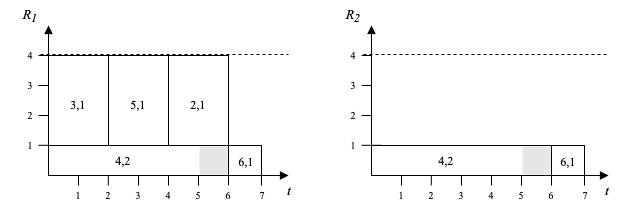
\includegraphics[width=1\textwidth]{assets/img/02_Grundlagen/ExampleProjectMRCPSP_ScheduleDelay.drawio.png}
    }
    \caption{MRCPSP Beispiel-Zeitplan mit einer Aktivitätsstörung von $\Delta_4$ = 1} 
    \label{img:example_mrcpsp_schedule_activitydisturbance}
    \source{Eigene Darstellung}
\end{figure}

Eine weitere Art von Unsicherheiten stellen Störungen bei den erneuerbaren Ressourcen dar. Bei dieser Störungsart besteht die Annahme, dass die Anzahl der verfügbaren Ressourcen einer Ressourcenart $R_k$ zu einem Zeitpunkt $t$ über die Differenz $\Delta^\rho_k \in \mathbb{N}$ reduziert wird. Über $t + \delta_t$ wird angegeben, ab welchem Zeitpunkt die erneuerbaren Ressourcenarten wieder komplett zur Verfügung stehen \cite[vgl.][S. 65 f.]{deblaere_reactive_2011}. Abbildung \ref{img:example_mrcpsp_schedule_resourcedisturbance} verdeutlicht die erneuerbaren Ressourcenstörungen. Im Zeitintervall $[4, 7]$ befindet sich eine erneuerbare Ressourcenstörung $\Delta^\rho_1 = 1$. Aktivität 2 kann somit nicht planmäßig ab Zeiteinheit 4 gestartet werden, da durch die Störung nicht genügend erneuerbare Ressourcen für den ausgewählten Modus vorhanden sind. Somit muss entweder ein anderer Modus ausgewählt werden oder solange mit dem Start von Aktivität 2 gewartet werden, bis die erneuerbaren Ressourcen für die komplette Laufzeit der Aktivität wieder zur Verfügung stehen. Der Start der Ausführung wäre bei dem selektierten Modus ab $t = 5$ der Fall, da durch das Fertigstellen von Aktivität 4 eine erneuerbare Ressource $R_1$ freigegeben wird und somit die erforderliche Anzahl von Ressourcen ($r_{2,1,1} = 3$) zur Verfügung stehen. Dadurch kommt jedoch bei Aktivität 6 ein Startverzug von einer Zeiteinheit. Durch diese Störung erhöht sich der Makespan des Zeitplans aus Abbildung \ref{img:example_mrcpsp_schedule_resourcedisturbance} ($C_{max} = 8$) gegenüber dem Zeitplan aus Abbildung \ref{img:example_mrcpsp_schedule} ($C_{max} = 7$) um eine Zeiteinheit.

\begin{figure}[H]
    \centering
    \noindent\makebox[\textwidth]{%
    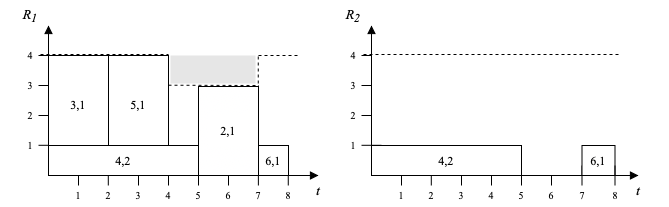
\includegraphics[width=1\textwidth]{assets/img/02_Grundlagen/ExampleProjectMRCPSP_ScheduleResourceDelay.drawio.png}
    }
    \caption{MRCPSP Beispiel-Zeitplan mit einer (erneuerbaren) Ressourcenstörung ab $t$ = 4 von $\Delta_1^\rho$ = 1, welche ab $t + \delta_t = 7$ normalisiert wird} 
    \label{img:example_mrcpsp_schedule_resourcedisturbance}
    \source{Eigene Darstellung}
\end{figure}

Das Ziel des (M)RCPSP besteht darin, den Zeitplan mit der geringsten Projektausführungsdauer zu finden. Der Umgang mit Unsicherheiten stellt zudem eine Herausforderung dar. \cite{brcic_resource_2012} beleuchtete in einer Erhebung einige Möglichkeiten zum Umgang des Unsicherheitsproblems für die stochastische Version des RCPSP. \\

Die naivste Herangehensweise mit Unsicherheiten umzugehen ist es diese bei der Zeitplanerstellung zu ignorieren. Diese Methode wird von \cite{brcic_resource_2012} als prädiktiv bezeichnet. Das Ignorieren von Unsicherheiten kann jedoch dazu führen, dass der Zeitplan durch Verspätungen stärker in Verzug kommt als bei anderen Herangehensweisen. \cite[vgl.][S. 404]{brcic_resource_2012} \\

Die proaktive Herangehensweise behandelt das Problem der Unsicherheiten, indem eine weitere Zielfunktion, nämlich die Robustheit eingeführt wird \cite[vgl.][S. 404]{brcic_resource_2012}. Die Robustheit gibt an, dass der Zeitplan mit geringfügigen Veränderungen (z. B. die der Unsicherheitszenarien) von Aktivitäten umgehen kann \cite[vgl.][S. 246]{khemakhem_efficient_2013}. \\

Die dritte Herangehensweise stellt die reaktiven Methoden dar. Diese reagieren direkt zum Zeitpunkt der Unsicherheit. Hierbei besteht die Möglichkeit, den Zeitplan ab der Unsicherheitsstelle zu reparieren oder gänzlich ab der Stelle der Unsicherheit einen neuen Zeitplan zu erstellen \cite[vgl.][S. 404 f.]{brcic_resource_2012}.  \\

In der Literatur werden prädiktive Verfahren auch als proaktive Verfahren bezeichnet und umgekehrt \cite[vgl.][S. 246]{khemakhem_efficient_2013}. Im Rahmen der Masterarbeit werden folglich die eingangs vorgestellten proaktiven Verfahren nun als prädiktive Verfahren behandelt, welche z. B. die Robustheit optimieren. Die eingangs vorgestellten prädiktiven Verfahren werden somit als proaktive Verfahren angesehen, welche z. B. Unsicherheiten ignorieren. Im Abschnitt  \ref{subsec:Praediktive_Methoden} werden die prädiktiven Methoden, repräsentierend durch die Robustheit,s konkreter vorgestellt. Die reaktiven Methoden, repräsentierend durch das Erzeugen von neuen Zeitplänen zu den Unsicherheitszeitpunkten, werden im Abschnitt \ref{subsec:Reaktive_Methoden} vorgestellt.

\subsubsection{Prädiktive Methoden}
\label{subsec:Praediktive_Methoden}

Eine Möglichkeit mit Unsicherheiten umzugehen stellt das vorausschauende Erstellen von Zeitplänen dar. Hierbei wird neben der Minimierung der Projektdauer $C_{max}$ eine weitere Zielfunktion eingeführt, nämlich die Maximierung der Robustheit $\Omega$. Die Robustheit gilt als die Maßeinheit, wie gut mit kleinen Änderungen innerhalb eines Zeitplans umgegangen werden kann, ohne dass die Projektdauer durch die Verspätung ansteigt \cite[vgl.][S. 246]{khemakhem_efficient_2013} \cite[vgl.][S. 177]{al-fawzan_bi-objective_2005}. \\

Eine mögliche Messung von Robustheit kann über die Summe aller freien Puffer der Aktivitäten definiert werden. Unter einem freien Puffer $s_j$ werden die Zeiteinheiten verstanden, die eingesetzt werden können, damit die unmittelbare Folgeaktivität nicht verzögert wird. Die Einhaltung der Ressourcenbeschränkung muss im Puffer dennoch berücksichtigt werden. Folglich ist die Robustheit über $\Omega = \sum_{j=1}^n s_j$ definiert. \cite[vgl.][S. 177]{al-fawzan_bi-objective_2005} \\

Der freie Puffer lässt sich über die frühsten und spätesten Start- bzw. Endzeitpunkte berechnen $s_j = LST_j - EST_j \Leftrightarrow s_j = LFT_j - EFT_j$. Während $EST_j$ und $EFT_j$ sich über den erstellten Zeitplan ablesen lassen, müssen $LST_j$ und $LFT_j$ über die Backward Recursive Prodecure berechnet werden \cite[vgl.][S. 181]{al-fawzan_bi-objective_2005}. \\

Bei dem \ac{rcpsp} Beispiel-Zeitplan $S^1$ aus Abbildung \ref{img:example_rcpsp_schedule} liegt die Robustheit bei $\Omega^1 = \sum_{j=1}^n s_j = 1$, da der einzige freie Puffer bei Aktivität $j_1$ liegt. Bei einer Verspätung von $\Delta_1 = 1$ würde es zu keiner Verspätung der Projektdauer $C_{max}$ kommen, da der Puffer genutzt werden kann. Sofern es bei einer anderen Aktivität zu einer Verspätung kommt, wird sich die Projektdauer $C_{max}$ verzögern. Ähnlich sieht es bei dem \ac{mrcpsp} Beispiel-Zeitplan $S^2$ aus Abbildung \ref{img:example_mrcpsp_schedule} aus, welcher ebenfalls einen Wert von $\Omega^2 = \sum_{j=1}^n s_j = s_4 = 1$ aufweist. Bei Nutzung des Puffers liegt nach dem Verspätungsszenario $\Delta_4 = 1$ die Robustheit bei $\Omega^{2'} = 0$ (vgl. Abbildung \ref{img:example_mrcpsp_schedule_activitydisturbance}). \\

Ein Zeitplan mit der gleichen Projektdauer $C_{max}$ kann unterschiedliche Robustheitswerte aufweisen und ist folglich für Unsicherheitsszenarien mehr oder weniger geeignet \cite[vgl.][S. 178]{al-fawzan_bi-objective_2005}. Beim prädiktiven Ansatz gilt es bei Zeitplänen mit identischer Projektdauer den mit dem höchsten Robustheitswert auszuwählen. \\

Die Robustheit lässt sich nicht nur über die Summe aller freien Puffer eines Zeitplans definieren. \cite{khemakhem_efficient_2013} vergleicht in seiner Publikation eine Menge von Robustmessungsfunktionen für das RCPSP und stellt das Prinzip der weighted slack functions (dt. gewichtete Pufferfunktionen) vor. Die Slack Function (dt. Pufferfunktion) stellt zum Beispiel die Summe der freien Puffer oder auch einen binärer Puffer dar \cite[vgl.][S. 253 f.]{khemakhem_efficient_2013}. Der Puffer kann anschließend über ein Weight (dt. Gewicht) multipliziert wird. Folglich wirkt sich ein Puffer für dominierende Aktivitäten stärker gegenüber einfachen Aktivitäten aus. Ein Weight kann die Anzahl von notwendigen Ressourcen, direkten oder totalen Nachfolgern einer Aktivität uvw. darstellen \cite[vgl.][S. 254 ff.]{khemakhem_efficient_2013}. Das Kombinieren von mehreren Weights ist ebenfalls möglich \cite[vgl.][S. 254 ff.]{khemakhem_efficient_2013}. \\

Tabelle \ref{tab:SlackFunctions} beinhaltet einen Ausschnitt von Slack Functions, welche von \cite{khemakhem_efficient_2013} vorgestellt wurden. Die Slack Functions können über die ebenfalls von \cite{khemakhem_efficient_2013} vorgestellten Weights aus Tabelle \ref{tab:Weights} gewichtet werden. \\

\begin{table}[H]
\centering
\resizebox{\textwidth}{!}{%
\begin{tabular}{r|l|l}
Slack Function & Beschreibung & Definition \\ \hline
$SF1$ & Summe von freien Puffern & $\sum_{j=1}^n s_j$ \\ \hline
$SF2$ & Summe von binären Puffern & $\sum_{j=1}^n \alpha$ mit $\alpha = \left\{\begin{array}{ll} 
        1 & \text{wenn $s_j > 0$} \\
        0 & \text{sonst} \\
     \end{array}\right. $ \\ \hline
$SF3$ & \begin{tabular}[c]{@{}l@{}}Minimum zwischen freien Puffer und \\ Bruchteil der Aktivitätsdauer $d_j$\end{tabular} &          $\sum_{j=1}^n \min (s_j, frac * d_j) $ mit $frac \in (0, 1) $  \\ \hline
$SF4$ & Funktion zum Verringern des freien Puffers & $\sum_{i=1}^{s_j} e^{-i}$ \\ \hline
... & ... & ...       
\end{tabular}
}%

\caption{Definitionen von Slack Functions zur Robustheitsmessung}
\label{tab:SlackFunctions}
\source{In Anlehnung an \cite[S. 254]{khemakhem_efficient_2013}}
\end{table}

\begin{table}[H]
\centering
\resizebox{0.7\textwidth}{!}{%
\begin{tabular}{r|l|l}
Weight & Beschreibung & Definition \\ \hline
$W1$ & Anzahl der direkten Nachfolger & $NDS_j$ \\ \hline
$W2$ & Anzahl der benötigten Ressourcen & $\sum_{k=1}^{K} r_{i,k}$ \\ \hline
$W3$ & Kombination von $W1$ und $W2$ & $NDS_j *  \sum_{k=1}^{K} r_{i,k}$\\ \hline
$W4$ & Anzahl der totalen Nachfolger & $NS_j$\\ \hline
... & ... & ...       
\end{tabular}
}%

\caption{Definitionen von Weights für die Gewichtung der Slacks innerhalb der Slack Functions zur Robustsheitmessung}
\label{tab:Weights}
\source{In Anlehnung an \cite[S. 255]{khemakhem_efficient_2013}}
\end{table}

Durch das Auswählen unterschiedlicher Slack Functions und Weights können eine Vielzahl von Robustheitsfunktionen hergeleitet werden. Eine Robustheitsfunktion $\Omega$, welche die Slack Function $SF2$ mit dem Weight $W1$ vorsieht, würde gemäß \cite{khemakhem_efficient_2013} wie folgt definiert sein: $\Omega^{SF2}_{W1} = \sum_{j=1}^n \alpha * NDS_j$. 

\subsubsection{Reaktive Methoden} \label{subsec:Reaktive_Methoden}

Unter reaktiven Methoden werden Verfahren verstanden, welche zum Zeitpunkt der Unsicherheit direkt reagieren, um so Verspätungen innerhalb der Projektdauer $C_{max}$ zu minimieren. \cite[vgl.][S. 404 f.]{brcic_resource_2012}. \\

Ein reaktiver Ansatz besteht darin, einen bestehenden Zeitplan zu einem Unsicherheitszeitpunkt zu reparieren. Hierbei werden zwischen proaktiven-reaktiven und prädiktiven-reaktiven Verfahren unterschieden. Diese Klassifizierung hängt von dem Baseline Schedule (zu dt. Basiszeitplan) ab, welcher initial festzulegen ist. Bei einem proaktiven-reaktiven Verfahren wird ein optimaler Zeitplan anhand der minimalen Projektdauer $C_{max}$ ausgewählt, während beim prädiktiven-reaktiven Verfahren ein optimaler Zeitplan sowohl anhand der minimalen Projektdauer $C_{max}$, als auch an einem weiteren Kriterium, wie die maximale Robustheit $\Omega$ ausgewählt wird \cite[vgl.][S. 404 f.]{brcic_resource_2012}. \\

Beim Reparieren gilt es zum Unsicherheitszeitpunkt neue Zeitpläne zu finden, welche zum einen gültig sind und zum anderen nah an dem Basiszeitplan liegen. Für das Finden von solchen Zeitplänen ist die Zielfunktion $\mathcal{C} = \sum_{i \in N} w_i | s_i' - s_i| + \sum_{i \in N} c_{im'_i}$ vorgesehen, welche die Rescheduling Kosten darstellen die es zu minimieren gilt. Hierbei stellen $s_i$ die Startzeitpunkte der Aktivitäten des Basiszeitplans und $s_i'$ die Startzeitpunkte für die Aktivitäten innerhalb des reparierenden Zeitplans dar. $w_i$ sind Inflexibilitätsgewichte, welche die Intensität von Aktivitätsstartabweichungen bestimmen. Im zweiten Teil der Zielfunktionen werden die Moduswechselkosten $c_{im'_i}$ aller Aktivitäten aufaddiert. Diese betragen $c_{im'_i} = 0$, wenn der Modus für eine Aktivität zum Basiszeitplan nicht gewechselt wird. Die Inflexibilitätsgewichte $w_i$ und die Moduswechselkosten $c_{im'_i}$ können im Vorfeld für einen Projektplan bestimmt werden. Mit diesen Werten ist es in der Praxis somit möglich, eher komplexere Änderungen dahingehend zu bestrafen, sodass diese für Folgezeitpläne weniger selektiert werden. \cite[vgl.][S. 5 f.]{deblaere_exact_2008}\\

% Das Reparieren kann über das Erstellen von neuen Zeitplänen zum Zeitpunkt der Unsicherheit sichergestellt werden. Hierbei werden die vorher durchlaufenen Aktivitäten und Modi \glqq{}eingefroren\grqq{}, da diese sich in der Vergangenheit nicht mehr ändern lassen. Die Folgeaktivitäten- und Modi werden anschließend ausgewechselt, so dass die Projektdauer $C_{max}$ minimal bleibt. Der Nachteil liegt darin, dass dieses Verfahren durch die NP-Vollständigkeit zwischen den Unsicherheiten zeitintensiv ist und zudem signifikante Änderungen zwischen dem Basiszeitplan und dem geänderten Zeitplan auftreten können. \cite[vgl.][S. 405]{brcic_resource_2012}. \\

Eine weitere Kategorie von reaktiven Methoden stellen die dynamischen Scheduling Methoden dar. Diese basieren nicht auf einem Basiszeitplan und erstellen Zeitpläne zur Laufzeit mithilfe von Regeln. \cite[S. 404]{brcic_resource_2012} Diese Masterthesis beschränkt sich im Rahmen der reaktiven Verfahren mit dem Reparieren von Zeitplänen anhand eines Basisplans. 